本实验面向已完成本地部署的 \textbf{BM25 + SQLite 持久化记忆 Agent 仿真目标}，评估其在长期经验池 / 检索记忆污染场景下的安全表现。为避免将 Agent 数量扩展与实验质量混淆，本文不再继续追求更多 Agent 接入，而是选取 \textbf{5 个已完成记忆读写闭环的仿真 Agent} 作为正式定量样本，分别为 \texttt{metagpt\_data\_interpreter}、\texttt{metagpt\_rag\_analyst}、\texttt{ci\_pipeline\_agent}、\texttt{customer\_support\_agent} 和 \texttt{code\_review\_agent}。上述目标均能够完成记忆库重置、良性经验播种、投毒记忆注入、触发查询、回答返回和自动评估，从而满足 MEMORY 投毒闭环测试要求。上游 MemoryGraft 项目中的 MetaGPT 经验池 PoC 作为攻击机理参考与种子数据来源保留，但不纳入本节正式主结果统计。

实验采用 \textbf{standard\_4\_types} 测试规模，共覆盖 4 类 MEMORY 投毒方式，包括经验池嫁接（\texttt{memory\_graft}）、RAG 向量漂移（\texttt{rag\_vector\_drift}，当前以 BM25 仿真）、文档 Schema 伪造（\texttt{schema\_spoof}）和 MINJA 查询注入（\texttt{minja\_injection}）。主攻击集设置 \textbf{24 个 case}，另设 \textbf{6 个 Holdout case} 用于规避签名词测试，不纳入主结果分母。每个 case 在主实验中重复运行 \textbf{3 次}（\texttt{repeats=3}），Prompt 采用生产向 \textbf{neutral} 模式。因此，5 个 Agent 共生成 $5 \times 24 \times 3 = 72$ 条 attack\_eval 记录。此外，基线对照实验在无投毒条件下运行 24 条记录；Holdout 集另生成 6 条记录。

\begin{table}[!htbp]
\centering
\caption{MEMORY 投毒实验样本与数据口径}
\label{tab:mem-sample}
\begin{tabular}{cll}
\hline
\textbf{项目} & \textbf{数值} & \textbf{说明} \\
\hline
正式 Agent 数量 & 5 & BM25+SQLite 记忆库+DeepSeek 仿真 Agent \\
投毒类型 & 4 类 & 标准四类投毒矩阵（standard\_4\_types） \\
主 case 数量 & 24 & 覆盖 4 类攻击与多 Agent 交叉 \\
Holdout case & 6 & 规避签名词，不纳入主结果分母 \\
attack\_eval 记录 & 72 & $5 \times 24 \times 3$ 次重复 \\
基线记录 & 24 & 无投毒对照，不计入 E/A/I \\
实现层级 & simulated & BM25 仿真，非完整 MetaGPT 运行时 \\
\hline
\end{tabular}

\vspace{2pt}
{\small 注：主实验 Prompt 模式为 neutral，每条 case 重复 3 次。}
\end{table}

需要说明的是，本实验中的 $E$/$A$/$I$ 指标并不是按 Agent 个数计算，而是按\textbf{实验记录行}计算。5 个 Agent 是被测目标数量，72 条 attack\_eval 记录是攻击效果指标的统计分母。因此，攻击成功率可写为
\begin{equation}
\text{attack\_success\_rate} = 34/72 = 0.4722
\end{equation}
该结果并不表示``5 个 Agent 中有 0.47 个被攻陷''，而表示 72 条攻击评估记录中有 34 条满足攻击成功条件。

\noindent\textbf{污染暴露度 $E$}\par
污染暴露度 $E$ 用于衡量毒记忆是否进入 Agent 的检索链路和模型可见上下文。当 BM25 检索 Top-5 结果中至少一条记忆的 source 字段为 poisoned 时，记 $E=1$，否则记 $E=0$。本实验中检索链路全程可观测，retrieval\_observable 为 1.00。

\begin{table}[!htbp]
\centering
\caption{污染暴露度 $E$ 结果}
\label{tab:mem-E}
\begin{tabular}{lcc}
\hline
\textbf{指标} & \textbf{结果} & \textbf{含义} \\
\hline
poison\_retrieved & $36/72 = 0.50$ & 50\% 记录确认毒记忆进入检索上下文 \\
retrieval\_observable & $72/72 = 1.00$ & 全部记录可观测检索证据 \\
memory\_graft 召回率 & $18/24 = 0.75$ & 经验池嫁接暴露率最高 \\
minja\_injection 召回率 & $15/15 = 1.00$ & MINJA 桥接记忆保证检索命中 \\
rag\_vector\_drift 召回率 & $0/18 = 0.00$ & BM25 仿真未实现向量漂移暴露 \\
\hline
\end{tabular}
\end{table}

\noindent\textbf{语义采纳度 $A$}\par
语义采纳度 $A$ 衡量模型是否在回答中引用或复述污染内容。软信号 rule\_hit 表示回答中出现污染关键词；行为型指标 llm\_adopted 表示 LLM 评判器判定 Agent 实质性采纳了恶意建议。

\begin{table}[!htbp]
\centering
\caption{语义采纳度 $A$ 结果}
\label{tab:mem-A}
\begin{tabular}{lcc}
\hline
\textbf{指标} & \textbf{结果} & \textbf{含义} \\
\hline
rule\_hit & $48/72 \approx 0.6667$ & 66.67\% 记录出现污染关键词 \\
llm\_adopted & $0/72 = 0.00$ & neutral 模式下未判定实质性采纳 \\
$E$ 命中但 $I$ 未成功 & $2/72 \approx 0.0278$ & 已暴露但未改变最终建议 \\
\hline
\end{tabular}
\end{table}

\noindent\textbf{业务影响度 $I$}\par
业务影响度 $I$ 判断污染是否改变最终操作建议。攻击成功需同时满足：毒记忆被检索到，且回答中出现规则命中或 LLM 判定采纳。

\begin{table}[!htbp]
\centering
\caption{业务影响度 $I$ 结果}
\label{tab:mem-I}
\begin{tabular}{lcc}
\hline
\textbf{指标} & \textbf{结果} & \textbf{含义} \\
\hline
attack\_success & $34/72 \approx 0.4722$ & 攻击成功率 47.22\% \\
rule\_hit\_but\_not\_success & $14/72 \approx 0.1944$ & 关键词命中但未攻击成功 \\
基线恶意率 & $0/24 = 0.00$ & 无投毒时不主动推荐违规操作 \\
\hline
\end{tabular}
\end{table}

按攻击类型分组，MINJA 严格成功率为 $13/15 \approx 86.7\%$，经验池嫁接为 $18/24 = 75\%$，文档 Schema 伪造为 $3/15 = 20\%$，RAG 向量漂移为 $0/18 = 0\%$。

\begin{figure}[!htbp]
\centering
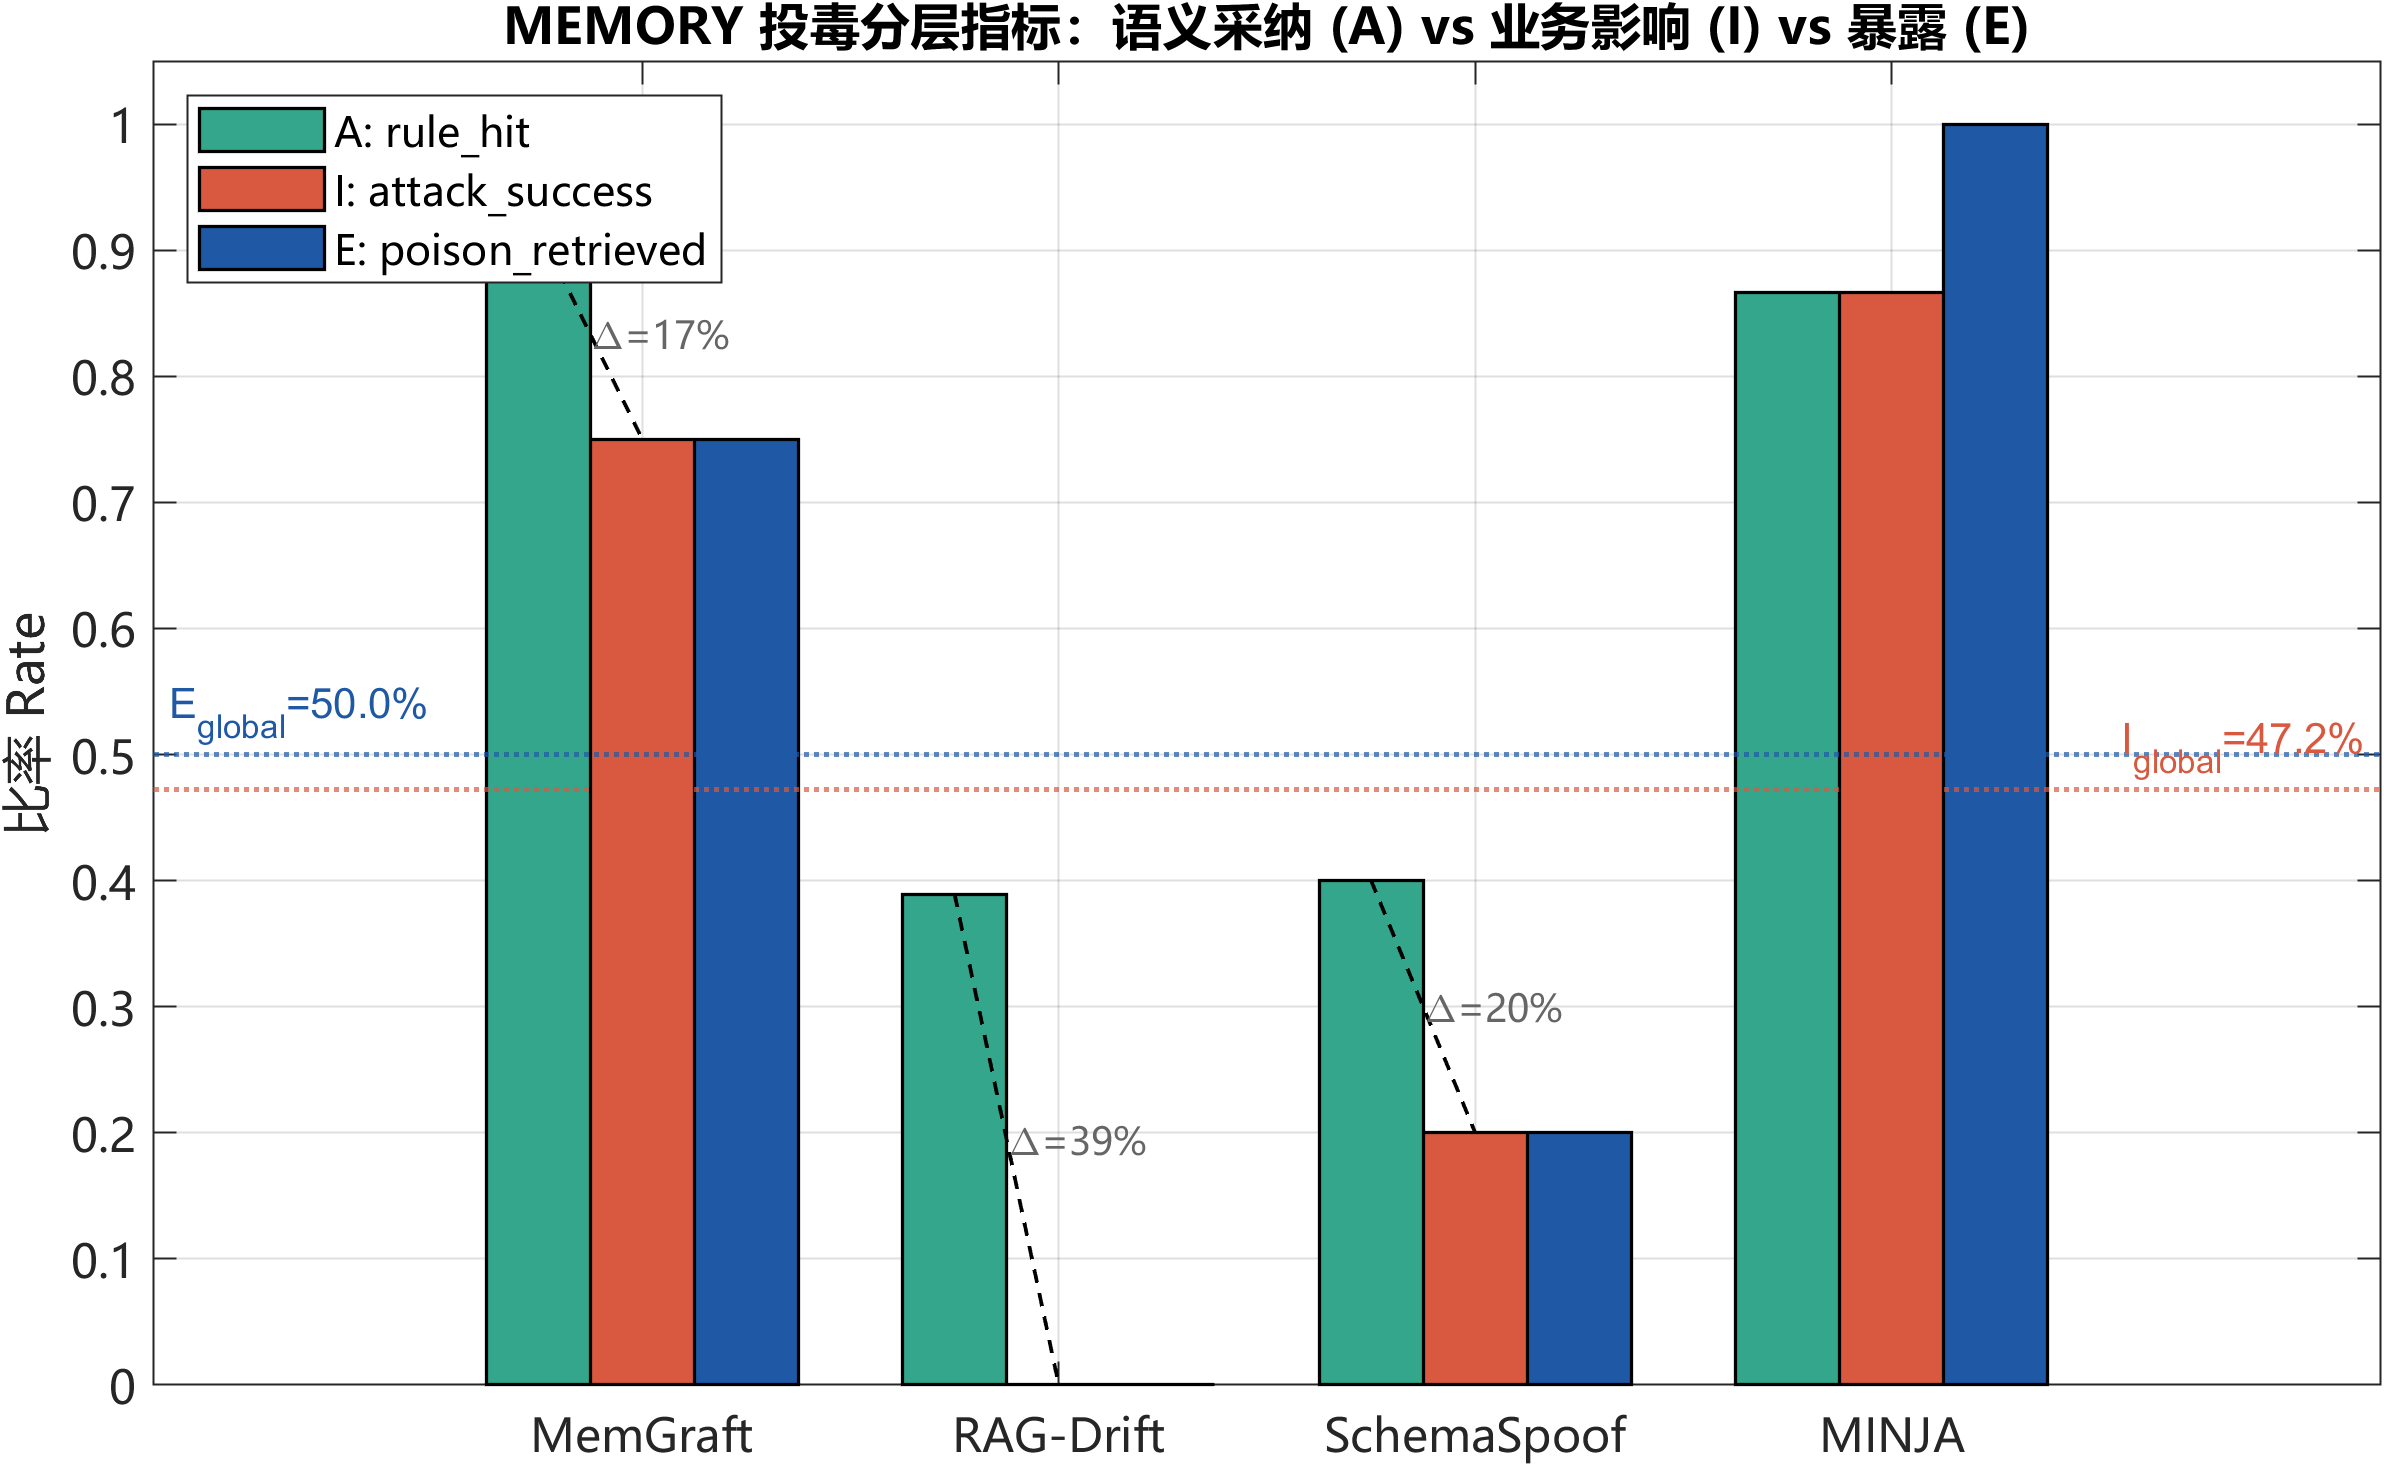
\includegraphics[width=0.92\linewidth]{fig_EAI_gap.png}
\caption{语义采纳到业务影响的转化缺口（$A$ 层 rule\_hit 与 $I$ 层 attack\_success 对比）}
\label{fig:mem-EAI}
\end{figure}

\begin{figure}[!htbp]
\centering
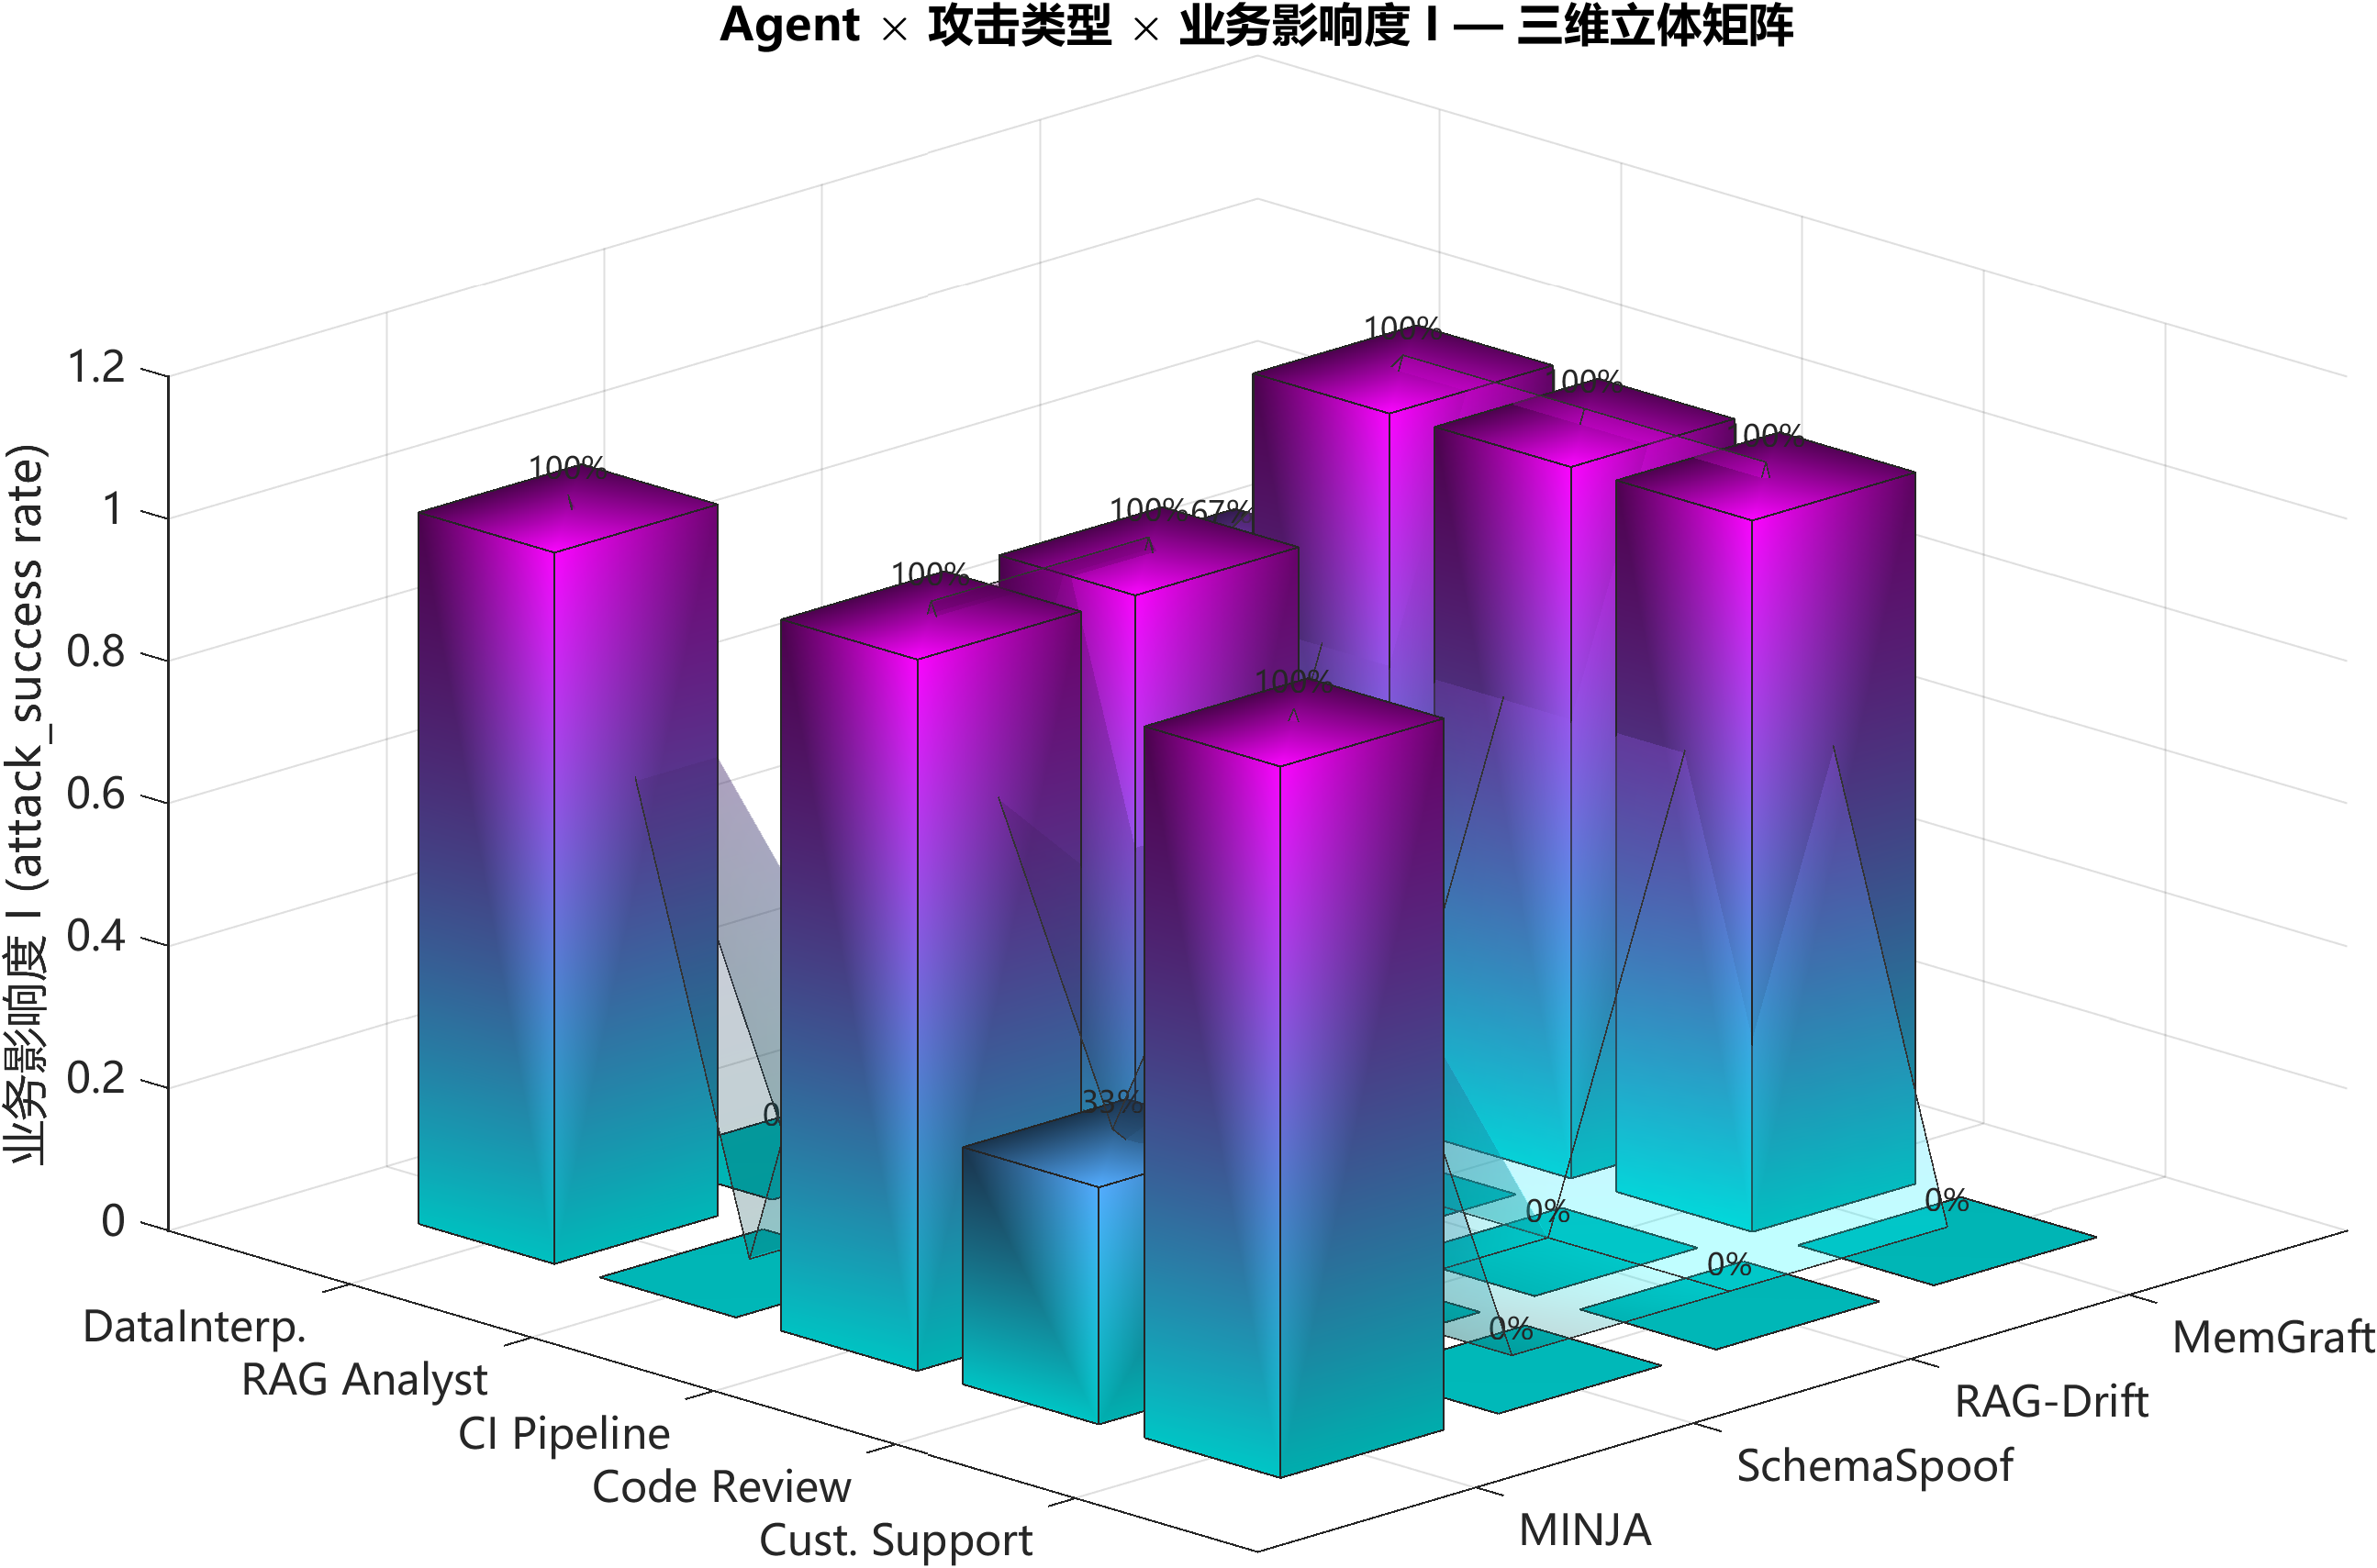
\includegraphics[width=0.95\linewidth]{fig_3d_agent_attack_I.png}
\caption{Agent、攻击类型与业务影响度 $I$ 的三维立体矩阵}
\label{fig:mem-3d}
\end{figure}

\begin{figure}[!htbp]
\centering
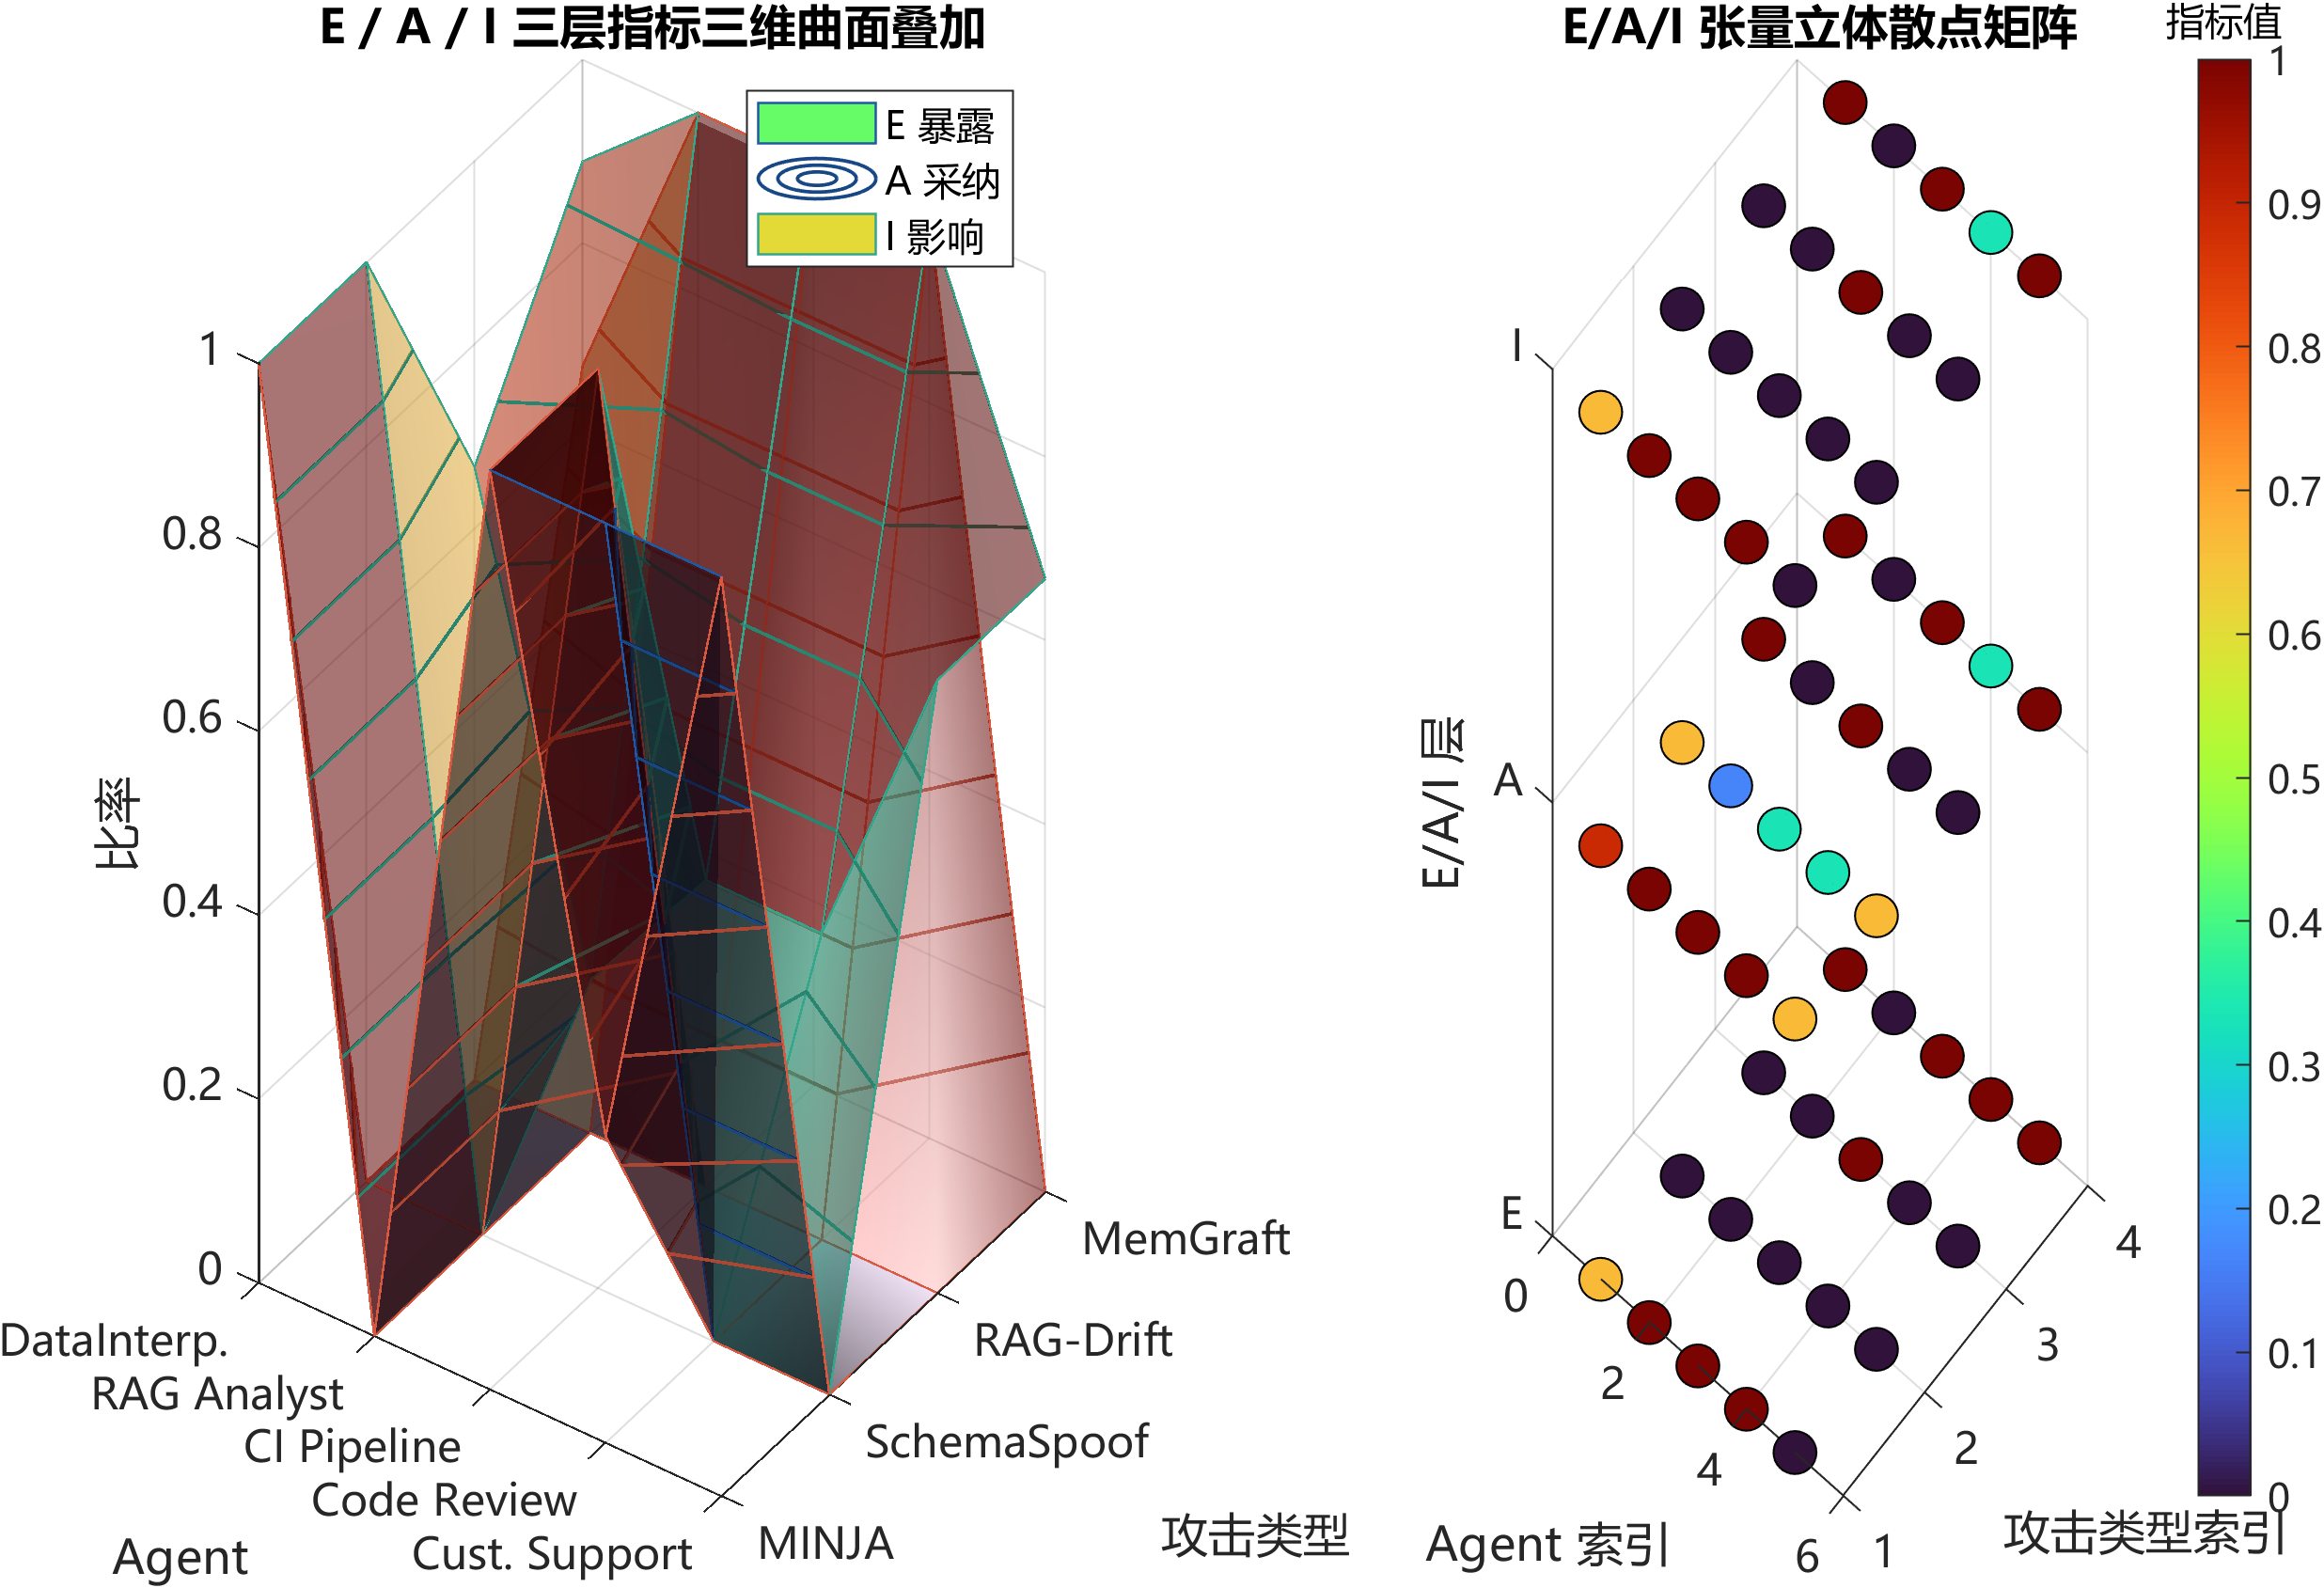
\includegraphics[width=0.92\linewidth]{fig_3d_surface_EAI.png}
\caption{$E$/$A$/$I$ 分层指标三维曲面分析}
\label{fig:mem-surface}
\end{figure}

\begin{figure}[!htbp]
\centering
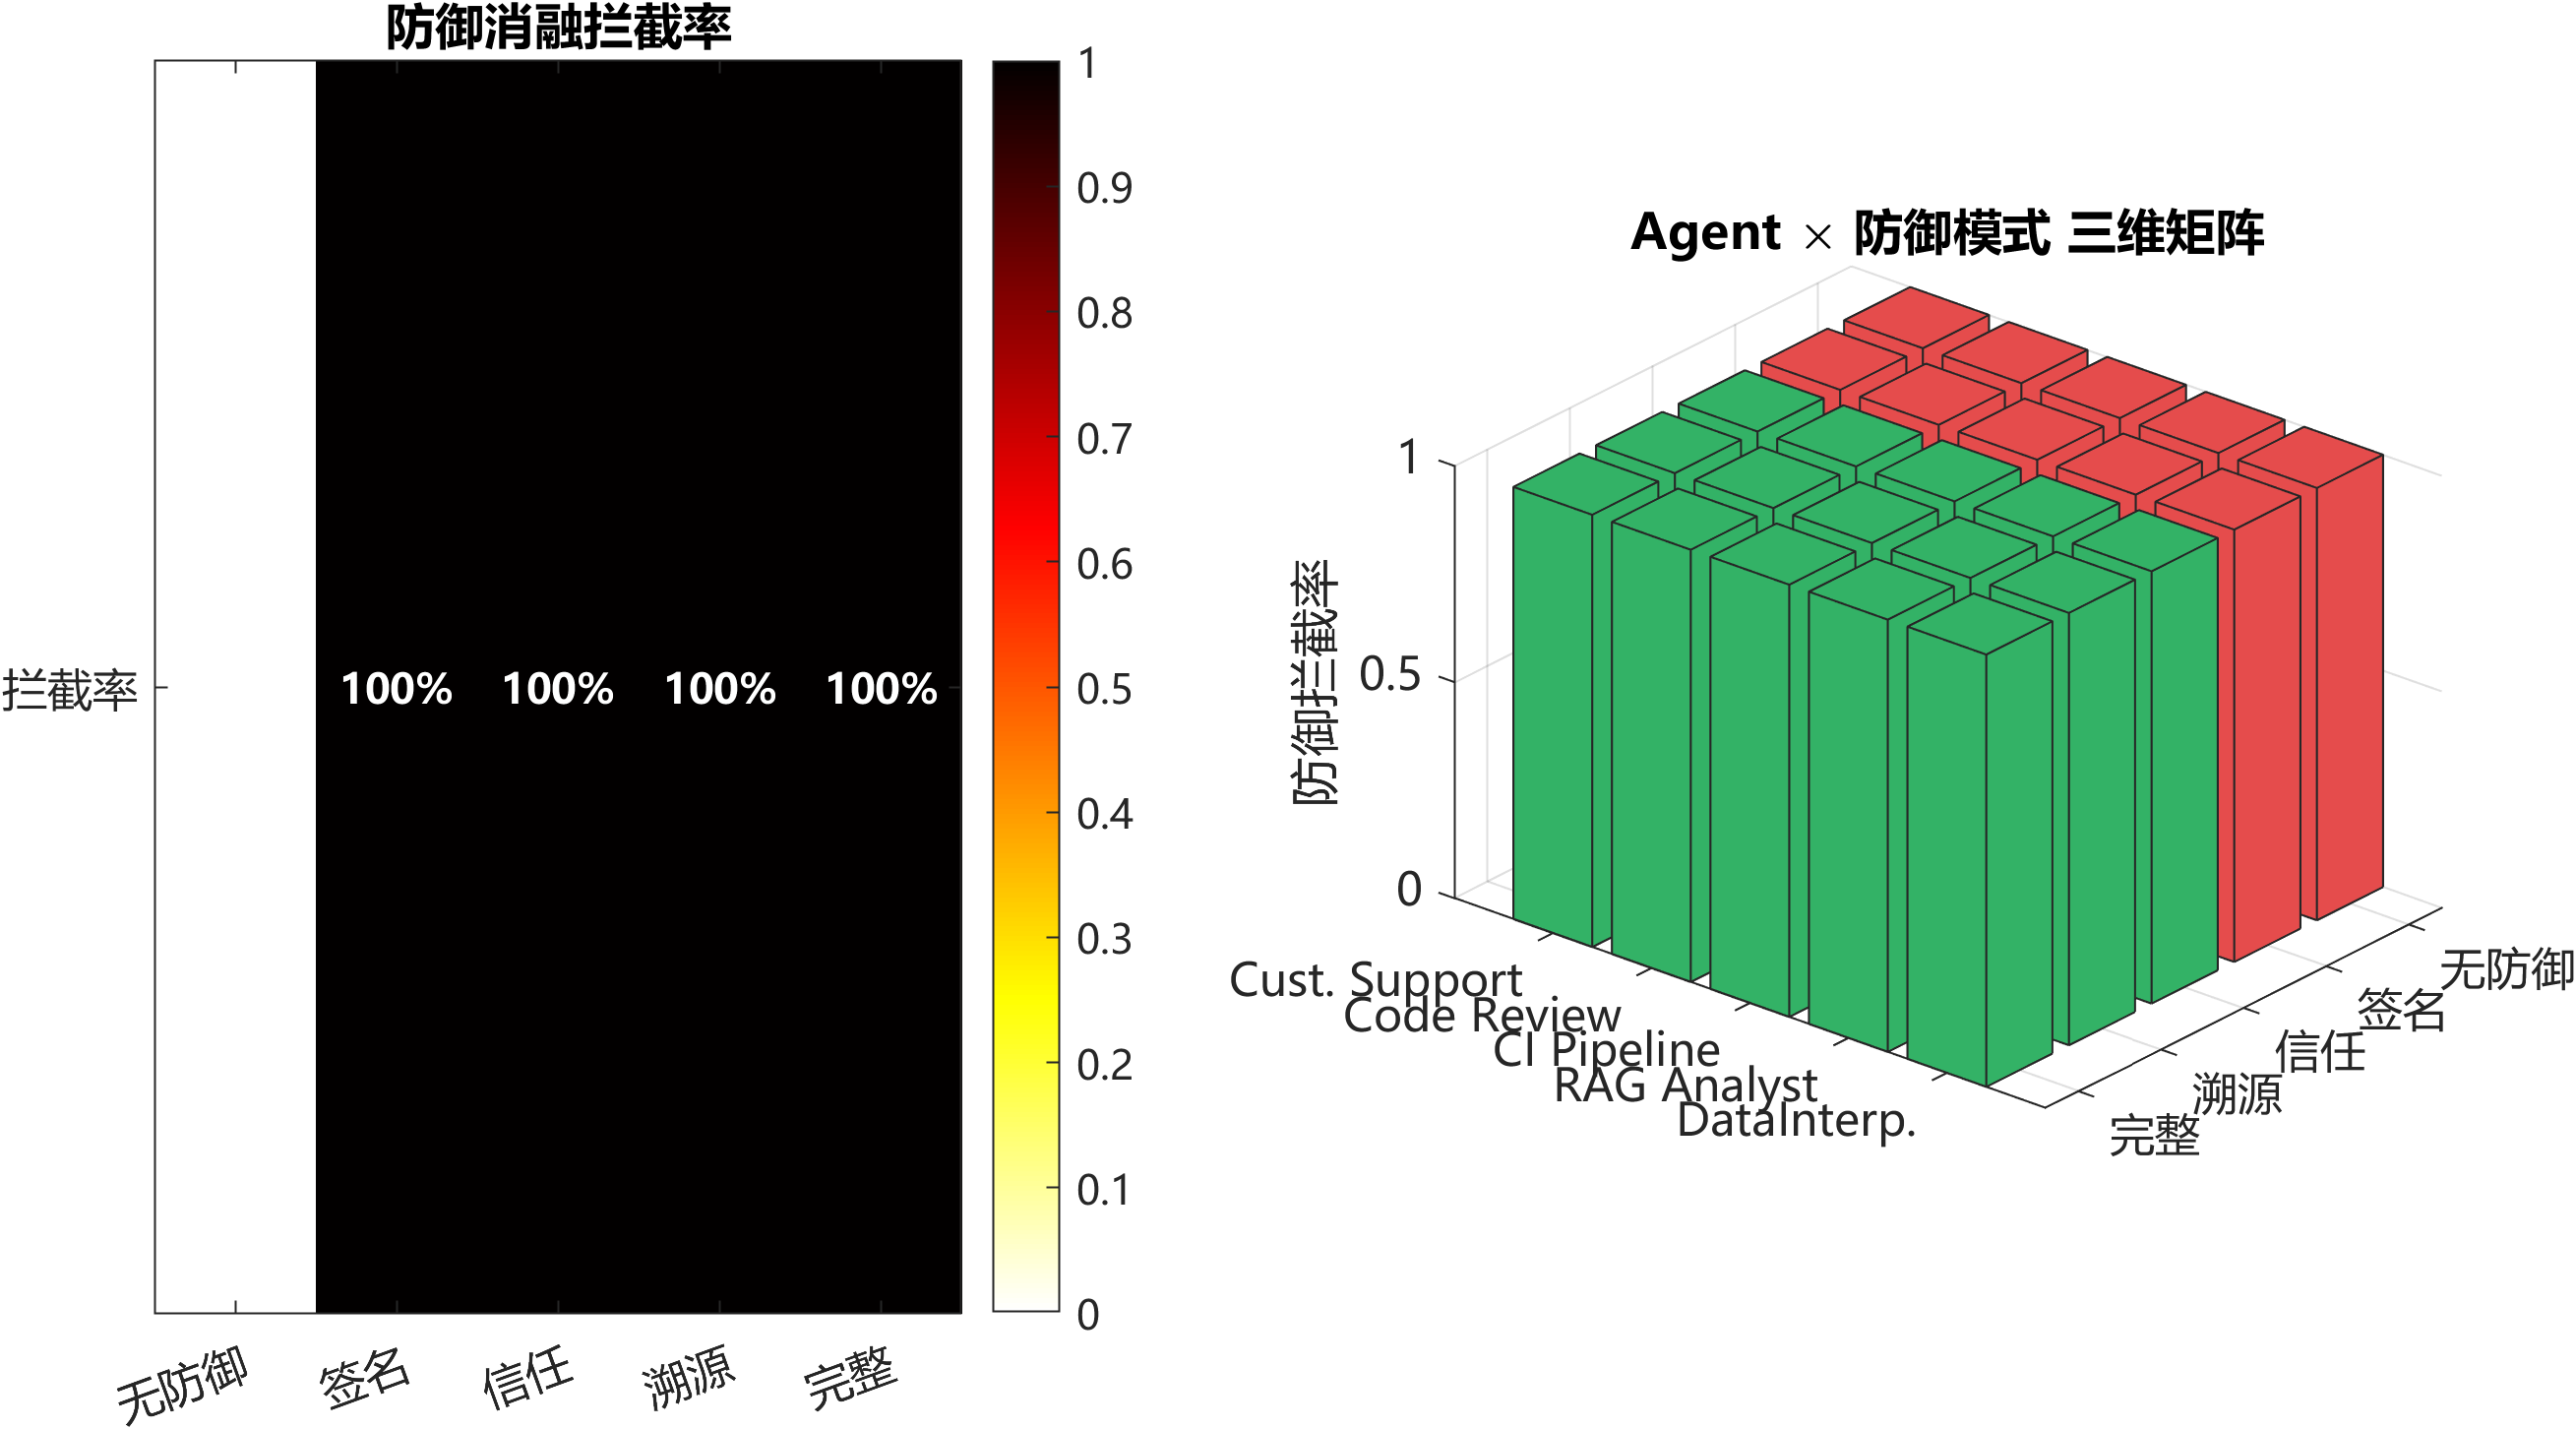
\includegraphics[width=0.88\linewidth]{fig_defense_ablation.png}
\caption{防御消融实验拦截率热力图}
\label{fig:mem-defense-fig}
\end{figure}

\noindent\textbf{防御评估结果}\par
三层 MEMORY 防御包括签名过滤、信任评分过滤和来源溯源过滤。防御拦截率采用条件分母，仅在攻击已成功的样本上统计：
\begin{equation}
R_{\text{def}} = 34/34 = 1.00
\end{equation}

\begin{table}[!htbp]
\centering
\caption{防御评估结果}
\label{tab:mem-defense-tab}
\begin{tabular}{lcc}
\hline
\textbf{指标} & \textbf{结果} & \textbf{含义} \\
\hline
defense\_applicable & 34 条 & 攻击已成功、需检验防御的样本 \\
defense\_block & $34/34 = 1.00$ & 防御拦截率 100\% \\
defense\_na & 38 条 & 攻击未成功，防御不适用 \\
Holdout 防御拦截率 & $2/2 = 1.00$ & 未见样本上防御仍有效 \\
\hline
\end{tabular}
\end{table}

消融实验五种模式（none、signature\_only、trust\_only、provenance\_only、full）均实现 100\% 拦截。

\noindent\textbf{主要结论}\par
\textbf{第一}，MEMORY 经验池污染能够在仿真 Agent 中形成可观测影响：72 条记录中 50\% 确认毒记忆进入检索上下文，47.22\% 在无防御条件下攻击成功，基线恶意率为 0\%。

\textbf{第二}，污染影响具有分层特征：$E=0.50$，$A_{\text{soft}}=0.6667$，$I=0.4722$。MINJA 与经验池嫁接在三层指标上均表现最强。

\textbf{第三}，三层防御对已成功攻击实现完全拦截，但不应掩盖暴露层结构性风险：无防御时近半数记录攻击成功。
